\appendix
%% Правка оформления ссылок на приложения:
%http://tex.stackexchange.com/questions/56839/chaptername-is-used-even-for-appendix-chapters-in-toc
%http://tex.stackexchange.com/questions/59349/table-of-contents-with-chapter-and-appendix
%% требует двойной компиляции
\addtocontents{toc}{\def\protect\cftchappresnum{\appendixname{} }%
\setlength{\cftchapnumwidth}{\widthof{\cftchapfont\appendixname~Ш\cftchapaftersnum}}%
}
%% Оформление заголовков приложений ближе к ГОСТ:
\sectionformat{\chapter}[display]{% Параметры заголовков разделов в тексте
    label=\chaptertitlename\ \thechapter,% (ГОСТ Р 2.105, 4.3.6)
    labelsep=20pt,
}
\renewcommand\thechapter{\Asbuk{chapter}} % Чтобы приложения русскими буквами нумеровались
   % Предварительные настройки для правильного подключения Приложений
\chapter{Листинги описаний концепций и типов} \label{AppendixA}

\lstinputlisting[language={Java},caption={Концепция "Цвет"},label={list:color}]{listings/Color.txt}

\lstinputlisting[language={Java},caption={Концепция "Ресурс"},label={list:resource}]{listings/Resource.txt}

\lstinputlisting[language={Java},caption={Концептуальный интерфейс "Держатель ресурсов"},label={list:IResouceCapturer}]{listings/IResouceCapturer.txt}

\lstinputlisting[language={Java},caption={Концептуальный интерфейс "Исполняемый"},label={list:IExecutable}]{listings/IExecutable.txt}

\lstinputlisting[language={Java},caption={Перечислимый тип "Тип связи"},label={list:ConnectionType}]{listings/ConnectionType.txt}

\lstinputlisting[language={Java},caption={Концепция "Место"},label={list:ConnectionType}]{listings/Place.txt}

\lstinputlisting[language={Java},caption={Концепция "Связь"},label={list:ConnectionType}]{listings/Connecton.txt}

\lstinputlisting[language={Java},caption={Концепция "Переход"},label={list:ConnectionType}]{listings/Transition.txt}

\lstinputlisting[language={Java},caption={Концепция "Сеть"},label={list:ConnectionType}]{listings/Net.txt}

\lstinputlisting[language={Java},caption={Концепция "Проект"},label={list:ConnectionType}]{listings/Project.txt}

\chapter{Описания ограничений} \label{AppendixB}

\lstinputlisting[language={Java},caption={Ограничения цвета},label={list:color-const}]{listings/constraints/Color.txt}

\lstinputlisting[language={Java},caption={Ограничения ресурсов},label={list:resource-const}]{listings/constraints/Resource.txt}

\lstinputlisting[language={Java},caption={Ограничения держателя ресурсов},label={list:IResouceCapturer-const}]{listings/constraints/IResourceCapturer.txt}

\lstinputlisting[language={Java},caption={Ограничения исполняемого интерфейса},label={list:IExecutable-const}]{listings/constraints/IExecutable.txt}

\lstinputlisting[language={Java},caption={Ограничения мест},label={list:ConnectionType-const}]{listings/constraints/Place.txt}

\lstinputlisting[language={Java},caption={Ограничения связей},label={list:ConnectionType-const}]{listings/constraints/Connection.txt}

\lstinputlisting[language={Java},caption={Ограничения сетей},label={list:ConnectionType-const}]{listings/constraints/Net.txt}

\lstinputlisting[language={Java},caption={Ограничения переходов},label={list:ConnectionType-const}]{listings/constraints/Transition.txt}

\chapter{Описания редакторов концепций} \label{AppendixC}

\begin{figure}[ht]
	\centering
	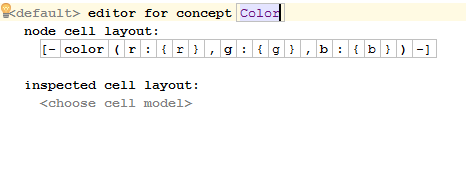
\includegraphics[width=0.7\linewidth]{images/editor/Color}
	\caption{Редактор цвета}
	\label{fig:color}
\end{figure}

\begin{figure}[ht]
	\centering
	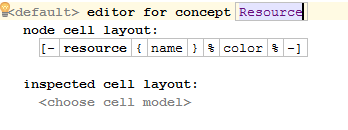
\includegraphics[width=0.7\linewidth]{images/editor/Resource}
	\caption{Редактор ресурсов}
	\label{fig:resource}
\end{figure}

\begin{figure}[ht]
	\centering
	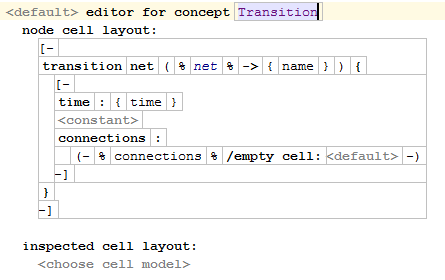
\includegraphics[width=0.7\linewidth]{images/editor/Transition}
	\caption{Редактор переходов}
	\label{fig:transition}
\end{figure}

\begin{figure}[ht]
	\centering
	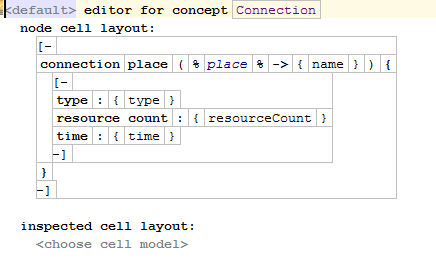
\includegraphics[width=0.7\linewidth]{images/editor/Connection}
	\caption{редактор связи}
	\label{fig:connection}
\end{figure}

\begin{figure}[ht]
	\centering
	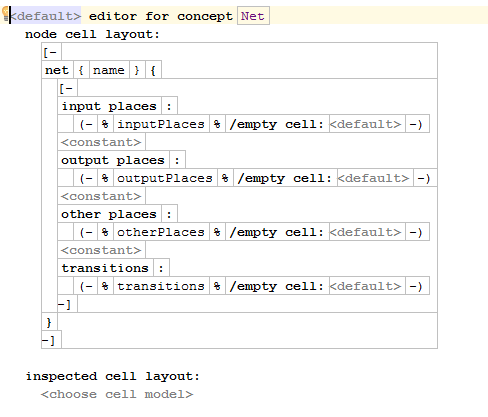
\includegraphics[width=0.7\linewidth]{images/editor/Net}
	\caption{Редактор сети}
	\label{fig:net}
\end{figure}

\begin{figure}[ht]
	\centering
	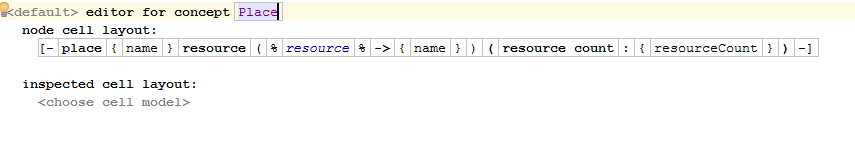
\includegraphics[width=0.7\linewidth]{images/editor/Place}
	\caption{Редактор места}
	\label{fig:place}
\end{figure}

\begin{figure}[ht]
	\centering
	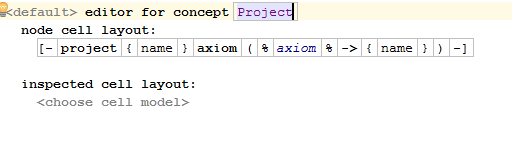
\includegraphics[width=0.7\linewidth]{images/editor/Project}
	\caption{Редактор проекта}
	\label{fig:project}
\end{figure}
